\documentclass[11pt]{article}
\usepackage[utf8]{inputenc}
\usepackage[margin=1in]{geometry}
\usepackage{enumitem}
\usepackage[T1]{fontenc}
\usepackage{lmodern}
\usepackage{textcomp}
\usepackage{microtype}
\usepackage{graphicx}
\usepackage{listings}
\usepackage{amsmath}
\usepackage{amssymb}
\usepackage{float}
\usepackage{booktabs}
\usepackage{parskip}
\usepackage{tabularx}
\usepackage{multirow}
\usepackage{tikz}
\usepackage{pgfplots}
\usepackage{xcolor}
\usepackage{hyperref}
\usepackage{cleveref}

% Define SI unit commands manually (siunitx alternative)
\newcommand{\SIval}[2]{#1\,#2}

\usetikzlibrary{shapes.geometric, arrows.meta, positioning, fit, calc}

\pgfplotsset{compat=1.18}

\hypersetup{
    colorlinks=true,
    linkcolor=blue,
    urlcolor=blue,
    citecolor=blue
}

\graphicspath{{images_src/}}

\lstset{basicstyle=\ttfamily\small, frame=single}

\title{Full Project Proposal:\\Transformer Robot}
\author{Gyan Edbert Zesiro (ID: 38600060) \and Ryan Edric Nashota (ID: 33508219)}
\date{\today}

\begin{document}
\maketitle
\tableofcontents
\newpage

%==============================================================================
\section{Concept}
%==============================================================================

\subsection{Goal and Vision}
We will build a simplified version of Caltech's Multi-Modal Mobility Morphobot (M4). The original M4 platform can transform between six locomotion modes; however, due to time and resource constraints, we narrow our scope to two high-impact modes:

\begin{itemize}
    \item \textbf{Ground Mode:} Agile wheeled driving suitable for indoor environments.
    \item \textbf{Flight Mode:} Short-hop quadrotor flight for obstacle traversal.
\end{itemize}

Our goal is to design and build a morphing robot that can switch between these two modes. We want to learn as much as possible from this project, so we will implement the following components from scratch:
\begin{itemize}
    \item Mechanical design and transformation mechanism
    \item Custom flight controller firmware
    \item Control system tuning
    \item Power distribution system
\end{itemize}

We recognize the complexity of designing these components. Building a flight controller alone requires deep understanding of control theory, sensor fusion, and embedded systems. However, this is our final year and we want to end it with a challenging project that pushes our abilities.

The vision is that by utilizing the same set of rotor-wheel appendages, we create a more versatile locomotion device capable of handling multiple scenarios. For example, the robot could drive efficiently through a building's corridors to survey damage, then switch to flight mode to cross a collapsed stairwell or navigate between floors through an open atrium.

\begin{figure}[H]
    \centering
    \includegraphics[width=0.5\textwidth]{m4_caltech.png}
    \caption{Caltech's M4 Robot, the inspiration for our project. The M4 demonstrates six locomotion modes through appendage repurposing.}
    \label{fig:m4_reference}
\end{figure}

\subsection{Form Factor and Operating Concept}
The robot resembles a remote-control car with four motorized wheels arranged in an ``X'' pattern on a central frame. What makes it special is that each wheel is part of a convertible rotor-wheel pod: essentially a propeller enclosed in a protective duct with a tire attached to its outer rim.

When driving on the ground, the pods lock flat at 0\,$^\circ$ and the motors spin the tires like a normal RC car. When the robot needs to fly (to get over obstacles or climb stairs), the four pods tilt upward to a 90\,$^\circ$ angle, the propellers spin up, and the whole system transforms into a quadcopter. Since the robot will be heavy, our goal is to provide enough flight time to hop over barriers and reach new locations, not sustained high-altitude flight.

Switching between driving and flying modes should be quick, targeting under 10 seconds. The transformation happens through motorized linear actuators that move the arms into preset positions, with Hall-effect sensors providing feedback to confirm correct positioning. An operator controls everything from an RC controller, deciding when to drive and when to take flight based on obstacles ahead.

\begin{figure}[H]
    \centering
    \includegraphics[width=0.7\textwidth]{2modes.jpeg}
    \caption{Conceptual sketch of the Transformer Robot in Ground Mode (left) and Flight Mode (right). The rotor-wheel pods rotate 90 degrees to switch between locomotion modes.}
    \label{fig:two_modes}
\end{figure}

\subsection{Conceptual Interest and Motivation}
The most compelling idea is appendage repurposing, similar to how animals use their limbs for multiple functions. We must design a single electromechanical module that provides traction, thrust, and stabilization, echoing M4's research insight while staying achievable within MECH 421/423 constraints.

Both of us want to pursue further study in mobile robot navigation. Unlike typical drones or rovers whose navigation algorithms are well studied, a morphing robot presents new challenges in state estimation, control, and path planning. This project exposes us to topics we want to research in graduate school.

Finally, we think it is just cool. While this robot has practical applications in search-and-rescue, the real motivation is the challenge and learning experience. Even if the final prototype does not achieve full autonomous transitions, the process of designing the transformation mechanism, creating a working PCB, integrating control systems, and wrestling with state estimation problems will teach us more than building yet another standard quadcopter or RC car.

%==============================================================================
\section{Answers to Questions from Concept Proposal}
%==============================================================================

\begin{enumerate}[label=\textbf{Q\arabic*:}, leftmargin=0pt, itemsep=1.2em]

\item \textbf{What is the value of your product to the end-user?}

The added flexibility from multiple modes allows a single robot to handle various scenarios. Urban search-and-rescue teams gain a robot that can roll quietly through doorways and then quickly hop over collapsed stair segments to reach trapped occupants. The operator stays at street level, teleoperates wheeled inspection, and only flies when debris gaps appear. This approach minimizes battery use while preserving access flexibility, shortening mission timelines and reducing the number of specialized robots responders must deploy.

Beyond emergency response, this technology could find applications in space exploration (planetary rovers that can fly over obstacles), agriculture (ground surveys with aerial overviews), military reconnaissance (driving through urban environments and flying over barriers), and environmental monitoring (ground-level data collection with aerial mapping).

\begin{figure}[H]
    \centering
    \includegraphics[width=0.85\textwidth]{use_case.png}
    \caption{Search and rescue storyboard illustrating the value proposition. The robot drives through accessible areas and flies over obstacles, enabling a single device to navigate complex disaster environments.}
    \label{fig:use_case}
\end{figure}

For our demonstration, we will show that the robot can navigate through tight spaces that a typical drone cannot pass through by switching to wheeled mode.

\item \textbf{What is the closest alternative to your product?}

Since our project is inspired by Caltech's M4, their research represents the closest alternative. The M4 robot demonstrates six locomotion modes including wheeled driving, flying, walking, and tumbling.

Other academic prototypes include Caltech's ATMO (Aerially Transforming Morphobot), which uses four thrusters that double as wheels and can transform between quadcopter and ground rover modes using a single motor mechanism. Virginia Tech has developed a bistable morphing robot using shape memory alloy actuators that rapidly switches between flying and driving configurations in under 50 milliseconds.

Outside research prototypes, there is no direct commercial equivalent. The practical alternative is using two separate robots: a standard quadcopter for aerial reconnaissance and an RC car or small ground rover for close-up inspection. This is what most hobbyists and professional applications currently do, switching between devices based on terrain.

\item \textbf{What is the metric of success for your product? How will you measure it?}

We will declare success if the robot:
\begin{enumerate}[label=(\roman*)]
    \item Completes a ground-to-flight-to-ground cycle in under 20\,s
    \item Sustains 0.8\,m/s average speed in drive mode for 15\,m
    \item Performs a 5\,m horizontal flight hop carrying its full chassis
\end{enumerate}

We will use timing gates for transformation measurements, encoder logs for ground speed verification, and visual markers or motion capture for flight distance quantification.

\item \textbf{Pick one aspect to polish to a finished product.}

The mechanical morphing mechanism and locking system will reach a polished standard. This means:
\begin{itemize}
    \item Smooth bearing-supported hinges with minimal play
    \item Hidden wiring routed through the frame
    \item Positive locking detents that audibly click into position
    \item Protective covers that shield components during takeoff
\end{itemize}

A rough prototype with visible wobble, exposed wires, or detents that need hand assistance is explicitly unacceptable and will be engineered out through iterative design and cable management.

\item \textbf{Which aspects will you not develop to a finished product?}

Full autonomy will not be achieved, though we will implement enough for safe operation. We will run RC teleoperation and simple attitude stabilization, but we will not harden SLAM, obstacle avoidance, or object detection. Most movement will rely on manual operation.

Additionally, features requiring datasets and validation (such as machine learning models) will not be implemented due to time constraints and our limited experience running ML models on embedded systems.

\item \textbf{What is your most critical module and why?}

The convertible rotor-wheel pod (FC2) is most critical because it must satisfy conflicting requirements:
\begin{itemize}
    \item Structural stiffness for fast driving over bumps
    \item Low mass for adequate flight performance
    \item Precise alignment for vibration-free hover
\end{itemize}

Failure to meet any requirement instantly degrades both locomotion modes. We will prototype this module first, run torsion and balance tests, and only then replicate it across all four corners.

\item \textbf{What kind of data infrastructure will you need? How will you test it?}

Our data infrastructure will stream wheel encoder ticks, IMU data, actuator position, current draw, and controller state vectors over serial to a logging laptop. A Python-based logging system will archive every trial with timestamps.

We will inject mock data using software simulation to ensure the telemetry pipeline handles expected bandwidth. We will then run hardware-in-the-loop bench tests where the Teensy publishes synthetic data while actuators report real motion, verifying synchronization before field trials.

\end{enumerate}

%==============================================================================
\section{Overview of Functional Components}
%==============================================================================

The transformer robot is divided into five functional components, each addressing a specific subsystem. Table~\ref{tab:fc_overview} summarizes each FC with effort allocation and responsible team member.

\begin{table}[H]
\centering
\caption{Functional Components Overview}
\label{tab:fc_overview}
\begin{tabular}{@{}clcc@{}}
\toprule
\textbf{FC} & \textbf{Description} & \textbf{\% Effort} & \textbf{Lead} \\
\midrule
FC1 & Morphing Airframe and Transformation Mechanism & 25\% & Ryan \\
FC2 & Rotor-Wheel Pod Assembly & 20\% & Ryan \\
FC3 & Motor Driver and Power Electronics & 20\% & Gyan \\
FC4 & Flight Controller and Sensor Fusion & 20\% & Gyan \\
FC5 & Ground Station and Telemetry Interface & 15\% & Both \\
\bottomrule
\end{tabular}
\end{table}

Figure~\ref{fig:flow_chart} shows the subsystem organization, and Figure~\ref{fig:system_architecture} shows how the functional components interact.

\begin{figure}[H]
    \centering
    \includegraphics[width=0.65\textwidth]{flow_chart.png}
    \caption{Subsystem flow chart showing the major components and their relationships in the Transformer Robot.}
    \label{fig:flow_chart}
\end{figure}

\begin{figure}[H]
\centering
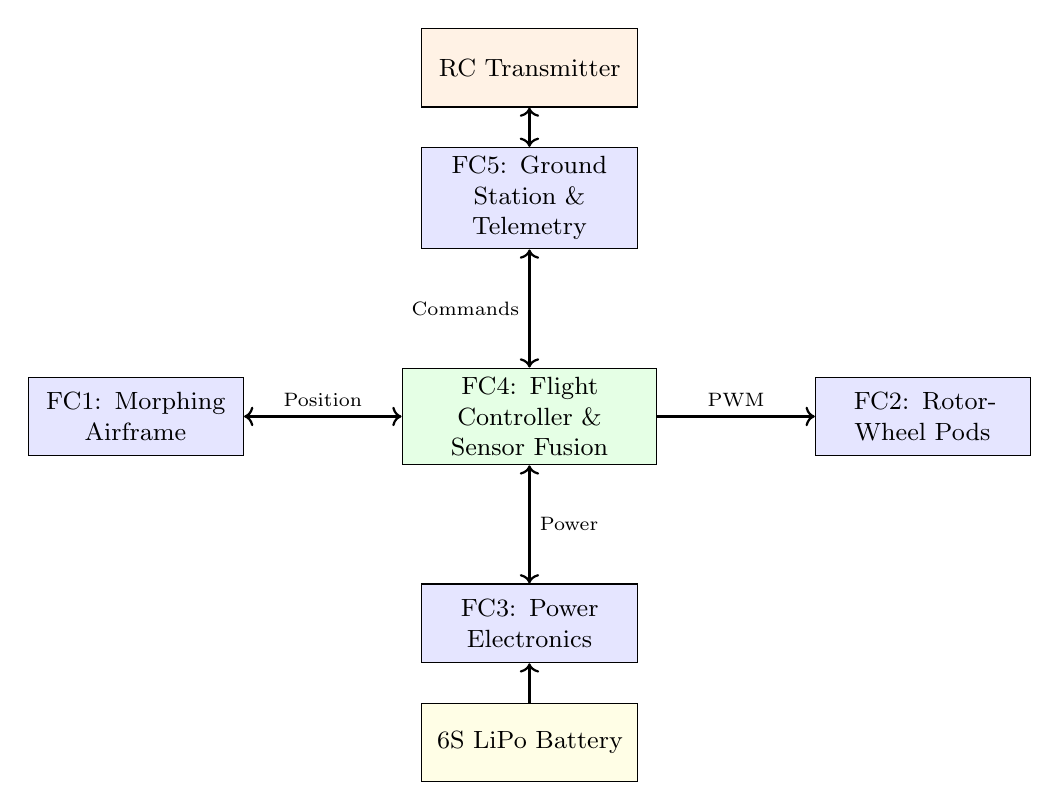
\begin{tikzpicture}[
    block/.style={rectangle, draw, fill=blue!10, text width=2.5cm, text centered, minimum height=1cm, font=\small},
    bigblock/.style={rectangle, draw, fill=green!10, text width=3cm, text centered, minimum height=1.2cm, font=\small},
    arrow/.style={-Stealth, thick},
    node distance=1.5cm
]

% Main controller
\node[bigblock] (fc4) {FC4: Flight Controller \& Sensor Fusion};

% Surrounding blocks
\node[block, above=of fc4] (fc5) {FC5: Ground Station \& Telemetry};
\node[block, left=2cm of fc4] (fc1) {FC1: Morphing Airframe};
\node[block, right=2cm of fc4] (fc2) {FC2: Rotor-Wheel Pods};
\node[block, below=of fc4] (fc3) {FC3: Power Electronics};

% Arrows
\draw[arrow, <->] (fc4) -- node[left, font=\scriptsize] {Commands} (fc5);
\draw[arrow, <->] (fc4) -- node[above, font=\scriptsize] {Position} (fc1);
\draw[arrow, ->] (fc4) -- node[above, font=\scriptsize] {PWM} (fc2);
\draw[arrow, <->] (fc4) -- node[right, font=\scriptsize] {Power} (fc3);

% External
\node[block, fill=orange!10, above=0.5cm of fc5] (rc) {RC Transmitter};
\draw[arrow, <->] (rc) -- (fc5);

\node[block, fill=yellow!10, below=0.5cm of fc3] (batt) {6S LiPo Battery};
\draw[arrow, ->] (batt) -- (fc3);

\end{tikzpicture}
\caption{System Architecture Block Diagram}
\label{fig:system_architecture}
\end{figure}

%==============================================================================
\section{Most Critical Module}
%==============================================================================

The most critical module is \textbf{FC2: Rotor-Wheel Pod Assembly}. This module faces the fundamental challenge of serving two masters: it must function as both a reliable ground wheel and an efficient aerial propulsion unit.

\subsection{Challenges}

\textbf{Conflicting Structural Requirements:} Ground driving subjects the pod to impact loads from bumps and curbs, demanding stiffness and durability. Flight requires minimal rotating mass for responsive attitude control and efficient hover. These requirements directly conflict.

\textbf{Vibration and Balance:} An unbalanced rotating assembly causes vibrations that degrade flight stability and accelerometer readings. The tire bonded to the propeller duct adds asymmetric mass that must be carefully balanced.

\textbf{Thermal Management:} Motors operating near their limits during flight generate significant heat. The enclosed duct design that protects the propeller also restricts airflow for cooling.

\textbf{Manufacturing Tolerances:} Four identical pods must be produced with tight tolerances. Variations in mass distribution or alignment between pods cause the flight controller to work harder to maintain stability.

\subsection{Work Done So Far}

We have completed preliminary CAD design of the rotor-wheel pod assembly, including:
\begin{itemize}
    \item 3D models of the duct, hub, and tire attachment mechanism
    \item Structural analysis of the arm connection points
    \item Initial motor and propeller selection based on thrust calculations
\end{itemize}

The CAD files are located in the project repository under \texttt{/CAD/Transforming+Quadcopter/}.

\subsection{Remaining Work}

\begin{enumerate}
    \item 3D print a single prototype pod for fit and function testing
    \item Conduct static thrust tests to verify motor and propeller performance
    \item Perform dynamic balancing using a balancing jig
    \item Measure vibration spectrum during operation
    \item Iterate on design based on test results
    \item Replicate the final design for all four pods
\end{enumerate}

Detailed development and test plans are provided in Section~\ref{sec:fc2}.

%==============================================================================
\section{FC1: Morphing Airframe and Transformation Mechanism}
\label{sec:fc1}
%==============================================================================

\subsection{Approach and Design}

The morphing airframe provides the structural backbone of the robot and houses the transformation mechanism that switches between ground and flight modes.

\textbf{Objective:} Create a rigid yet lightweight frame that supports all components and enables reliable, repeatable transformation between locomotion modes.

\textbf{Frame Construction:} The main chassis consists of two carbon fiber plates (2\,mm thickness, 300x200\,mm) forming top and bottom decks connected by aluminum standoffs. This sandwich construction provides excellent stiffness-to-weight ratio.

\textbf{Transformation Mechanism:} Each rotor-wheel pod is mounted on a pivoting arm. Linear actuators drive the arms between two positions:
\begin{itemize}
    \item Ground mode: Arms horizontal (0\,$^\circ$)
    \item Flight mode: Arms vertical (90\,$^\circ$)
\end{itemize}

\textbf{Position Feedback:} Hall-effect sensors at each pivot detect magnets embedded in the arms, providing binary feedback for locked positions. This allows the controller to verify successful transformation before enabling the appropriate control mode.

\begin{figure}[H]
    \centering
    \includegraphics[width=0.6\textwidth]{mechanism.jpeg}
    \caption{Preliminary concept sketch of the transformation mechanism showing the pivot arm and actuator arrangement.}
    \label{fig:mechanism_sketch}
\end{figure}

\begin{figure}[H]
\centering
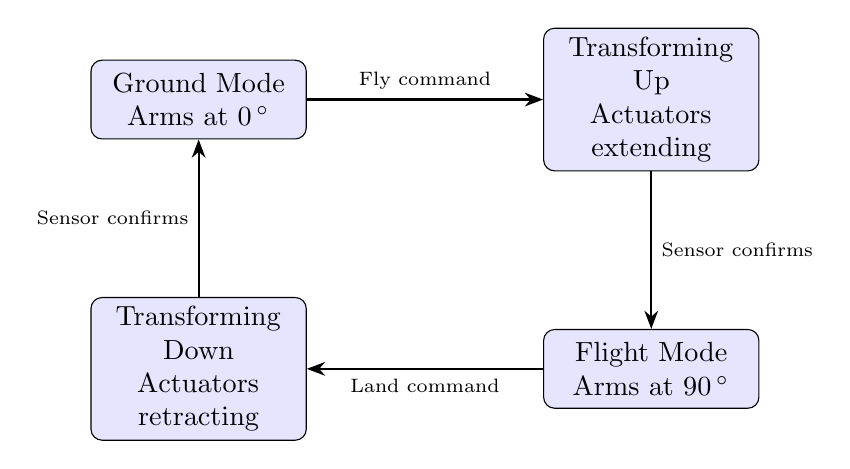
\begin{tikzpicture}[
    state/.style={rectangle, rounded corners, draw, fill=blue!10, text width=2.5cm, text centered, minimum height=1cm},
    arrow/.style={-Stealth, thick}
]

\node[state] (ground) {Ground Mode\\Arms at 0\,$^\circ$};
\node[state, right=3cm of ground] (trans_up) {Transforming Up\\Actuators extending};
\node[state, below=2cm of trans_up] (flight) {Flight Mode\\Arms at 90\,$^\circ$};
\node[state, left=3cm of flight] (trans_down) {Transforming Down\\Actuators retracting};

\draw[arrow] (ground) -- node[above, font=\scriptsize] {Fly command} (trans_up);
\draw[arrow] (trans_up) -- node[right, font=\scriptsize] {Sensor confirms} (flight);
\draw[arrow] (flight) -- node[below, font=\scriptsize] {Land command} (trans_down);
\draw[arrow] (trans_down) -- node[left, font=\scriptsize] {Sensor confirms} (ground);

\end{tikzpicture}
\caption{Transformation State Machine}
\label{fig:state_machine}
\end{figure}

\begin{figure}[H]
\centering
\fbox{\parbox{0.8\textwidth}{\centering\vspace{3cm}\textbf{[PLACEHOLDER: CAD Isometric View of Full Assembly]}\\\small Insert rendered image of complete robot assembly\vspace{3cm}}}
\caption{CAD Model: Isometric View of Transformer Robot Assembly}
\label{fig:cad_isometric}
\end{figure}

\subsection{Inputs and Outputs}

\begin{table}[H]
\centering
\caption{FC1 Inputs and Outputs}
\label{tab:fc1_io}
\begin{tabular}{@{}llll@{}}
\toprule
\textbf{Signal} & \textbf{Type} & \textbf{Range} & \textbf{Description} \\
\midrule
\multicolumn{4}{l}{\textit{Inputs}} \\
Transform\_Cmd & Digital & 0/1 & Command to initiate transformation \\
Target\_Mode & Digital & 0/1 & 0 = Ground, 1 = Flight \\
\midrule
\multicolumn{4}{l}{\textit{Outputs}} \\
Actuator\_PWM & PWM & 0--100\% & Drive signal to linear actuators \\
Actuator\_Dir & Digital & 0/1 & Direction control (extend/retract) \\
\midrule
\multicolumn{4}{l}{\textit{Feedback}} \\
Hall\_Ground & Digital & 0/1 & Ground position detected \\
Hall\_Flight & Digital & 0/1 & Flight position detected \\
Current\_Sense & Analog & 0--5\,V & Actuator current for stall detection \\
\bottomrule
\end{tabular}
\end{table}

\subsection{Parameters}

\begin{itemize}
    \item \textbf{Ground angle:} 0\,$^\circ$ (horizontal arms)
    \item \textbf{Flight angle:} 90\,$^\circ$ (vertical arms)
    \item \textbf{Actuator stroke:} 100\,mm
    \item \textbf{Actuator force:} 150\,N minimum (upgraded from initial 60\,N)
    \item \textbf{Actuator speed:} 15\,mm/s
    \item \textbf{Transformation timeout:} 10\,s maximum
    \item \textbf{Hall sensor threshold:} Digital with 5\,mm magnet proximity
\end{itemize}

The actuator force was increased from 60\,N after preliminary calculations showed the original specification was marginal for lifting the pod mass against gravity during transformation.

\subsection{Development Plan}

\begin{enumerate}
    \item Finalize frame CAD and generate DXF files for carbon fiber cutting
    \item Order carbon fiber plates and have them CNC cut
    \item 3D print mounting brackets and actuator housings in PLA
    \item Assemble frame with standoffs and verify dimensional accuracy
    \item Mount linear actuators and wire to DRV8871 drivers
    \item Install Hall-effect sensors and calibrate detection positions
    \item Write transformation control routine and integrate with main controller
    \item Conduct transformation cycle testing
\end{enumerate}

\subsection{Test Plan}

\begin{table}[H]
\centering
\caption{FC1 Test Plan}
\label{tab:fc1_tests}
\begin{tabular}{@{}lll@{}}
\toprule
\textbf{Test} & \textbf{Method} & \textbf{Success Criteria} \\
\midrule
Transformation Time & Stopwatch timing & $<$ 10\,s full cycle \\
Lock Engagement & Visual inspection & Audible click, no wobble \\
Position Accuracy & Protractor measurement & $\pm$2\,$^\circ$ of target \\
Cycle Fatigue & 100 transformation cycles & No mechanical degradation \\
Sensor Reliability & 50 detection tests & 100\% correct detection \\
\bottomrule
\end{tabular}
\end{table}

%==============================================================================
\section{FC2: Rotor-Wheel Pod Assembly}
\label{sec:fc2}
%==============================================================================

\subsection{Approach and Design}

The rotor-wheel pod is the defining feature of the transformer robot, serving as both wheel and propulsion unit.

\textbf{Objective:} Create a module that provides ground traction when horizontal and aerial thrust when vertical, using shared mechanical components.

\textbf{Pod Construction:} Each pod consists of:
\begin{itemize}
    \item \textbf{Brushless motor:} 2812 Pro 1100\,KV mounted at the center
    \item \textbf{Propeller:} 8-inch or 9-inch propeller attached to motor shaft
    \item \textbf{Duct:} 3D-printed shroud surrounding the propeller for protection and efficiency
    \item \textbf{Tire:} Rubber tire bonded to the outer rim of the duct
    \item \textbf{Hub:} Central hub connecting the pod to the pivot arm
\end{itemize}

\textbf{Operating Modes:}
\begin{itemize}
    \item \textbf{Ground mode:} Motor spins the entire pod assembly; tire contacts ground for traction
    \item \textbf{Flight mode:} Motor spins only the propeller; pod body remains stationary
\end{itemize}

A clutch mechanism (or separate drive motors) may be needed to decouple the propeller from the duct during ground operation. Initial prototypes will test both approaches.

\begin{figure}[H]
\centering
\fbox{\parbox{0.8\textwidth}{\centering\vspace{3cm}\textbf{[PLACEHOLDER: Exploded View of Rotor-Wheel Pod]}\\\small Insert CAD exploded view showing motor, propeller, duct, tire, and hub\vspace{3cm}}}
\caption{CAD Model: Exploded View of Rotor-Wheel Pod Assembly}
\label{fig:cad_pod_exploded}
\end{figure}

\subsection{Inputs and Outputs}

\begin{table}[H]
\centering
\caption{FC2 Inputs and Outputs}
\label{tab:fc2_io}
\begin{tabular}{@{}llll@{}}
\toprule
\textbf{Signal} & \textbf{Type} & \textbf{Range} & \textbf{Description} \\
\midrule
\multicolumn{4}{l}{\textit{Inputs (from FC4)}} \\
Motor\_PWM & PWM & 1000\,$\mu$s--2000\,$\mu$s & Throttle command to ESC \\
\midrule
\multicolumn{4}{l}{\textit{Outputs (mechanical)}} \\
Thrust (flight) & Force & 0--10\,N & Vertical thrust per pod \\
Torque (ground) & Torque & 0--0.5\,Nm & Drive torque at wheel \\
\midrule
\multicolumn{4}{l}{\textit{Feedback}} \\
RPM (optional) & Frequency & 0--15000\,RPM & Motor speed from ESC telemetry \\
\bottomrule
\end{tabular}
\end{table}

\subsection{Parameters}

\begin{itemize}
    \item \textbf{Motor KV rating:} 1100\,KV (RPM per volt)
    \item \textbf{Propeller size:} 8x4.5 or 9x5 inches (diameter x pitch)
    \item \textbf{Tire outer diameter:} 100\,mm
    \item \textbf{Duct inner clearance:} 2\,mm tip gap
    \item \textbf{Pod total mass:} Target $<$ 300\,g
    \item \textbf{Static thrust:} Target $>$ 800\,g per pod at full throttle
\end{itemize}

Propeller pitch affects both thrust and efficiency. Higher pitch provides more thrust but requires more power. We will test multiple propeller options to find the best balance.

\subsection{Development Plan}

\begin{enumerate}
    \item Finalize single pod CAD design
    \item 3D print duct and hub components
    \item Assemble prototype with motor and propeller (without tire initially)
    \item Conduct static thrust test on test stand
    \item Add tire and repeat thrust test to measure impact
    \item Perform dynamic balancing using a balancing jig
    \item Measure vibration spectrum with accelerometer
    \item Iterate design based on results
    \item Produce four matched pods for final assembly
\end{enumerate}

\subsection{Test Plan}

\begin{table}[H]
\centering
\caption{FC2 Test Plan}
\label{tab:fc2_tests}
\begin{tabular}{@{}lll@{}}
\toprule
\textbf{Test} & \textbf{Method} & \textbf{Success Criteria} \\
\midrule
Static Thrust & Load cell test stand & $>$ 800\,g per pod \\
Vibration & Accelerometer FFT & No dominant peaks $>$ 0.5\,g RMS \\
Balance & Balancing jig & $<$ 1\,g-cm imbalance \\
Thermal & Thermocouple on motor & $<$ 80\,$^\circ$C after 60\,s hover \\
Ground Traction & Tow force measurement & $>$ 2\,N traction force \\
\bottomrule
\end{tabular}
\end{table}

%==============================================================================
\section{FC3: Motor Driver and Power Electronics}
\label{sec:fc3}
%==============================================================================

\subsection{Approach and Design}

The power electronics subsystem manages energy distribution from the battery to all motors and provides regulated power for control electronics.

\textbf{Objective:} Deliver reliable power to all actuators while protecting against overcurrent, undervoltage, and reverse polarity conditions.

\textbf{Components:}
\begin{itemize}
    \item \textbf{Flight ESCs:} 4-in-1 45\,A ESC stack for the four flight motors
    \item \textbf{Drive ESCs:} Two 35\,A bidirectional ESCs for ground drive motors (5010 360\,KV)
    \item \textbf{Actuator drivers:} Two DRV8871 H-bridge modules for linear actuators
    \item \textbf{Voltage regulators:} Buck converters for 5\,V (logic) and 12\,V (actuators)
    \item \textbf{Power distribution:} Custom PCB with XT60 connectors
\end{itemize}

\begin{figure}[H]
\centering
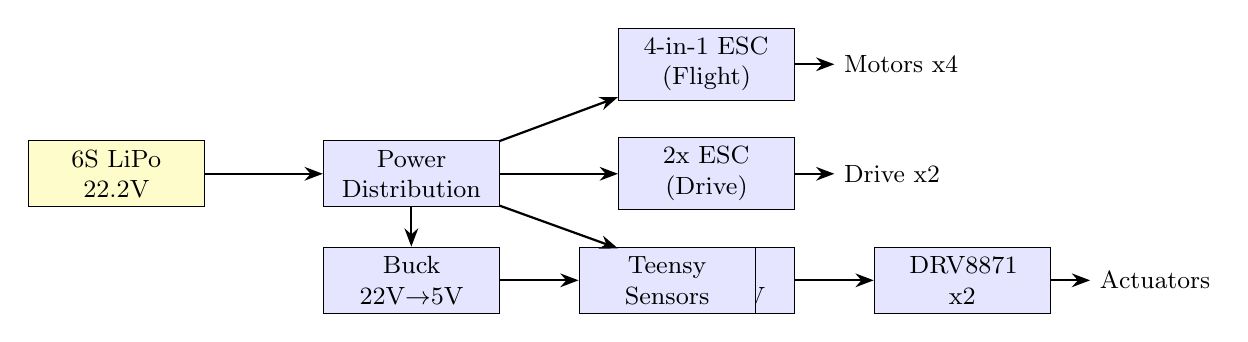
\begin{tikzpicture}[
    block/.style={rectangle, draw, fill=blue!10, text width=2cm, text centered, minimum height=0.8cm, font=\small},
    arrow/.style={-Stealth, thick},
    node distance=1cm
]

% Battery
\node[block, fill=yellow!20] (batt) {6S LiPo\\22.2V};

% Main distribution
\node[block, right=1.5cm of batt] (pdb) {Power\\Distribution};

% Branches
\node[block, above right=0.5cm and 1.5cm of pdb] (esc4) {4-in-1 ESC\\(Flight)};
\node[block, right=1.5cm of pdb] (esc2) {2x ESC\\(Drive)};
\node[block, below right=0.5cm and 1.5cm of pdb] (buck12) {Buck\\22V$\to$12V};

\node[block, right=1cm of buck12] (drv) {DRV8871\\x2};

\node[block, below=0.5cm of pdb] (buck5) {Buck\\22V$\to$5V};

\node[block, right=1cm of buck5] (logic) {Teensy\\Sensors};

% Motors
\node[right=0.5cm of esc4, font=\small] (m4) {Motors x4};
\node[right=0.5cm of esc2, font=\small] (m2) {Drive x2};
\node[right=0.5cm of drv, font=\small] (act) {Actuators};

% Arrows
\draw[arrow] (batt) -- (pdb);
\draw[arrow] (pdb) -- (esc4);
\draw[arrow] (pdb) -- (esc2);
\draw[arrow] (pdb) -- (buck12);
\draw[arrow] (pdb) -- (buck5);
\draw[arrow] (buck12) -- (drv);
\draw[arrow] (buck5) -- (logic);
\draw[arrow] (esc4) -- (m4);
\draw[arrow] (esc2) -- (m2);
\draw[arrow] (drv) -- (act);

\end{tikzpicture}
\caption{Power Distribution Diagram}
\label{fig:power_dist}
\end{figure}

\begin{figure}[H]
\centering
\fbox{\parbox{0.8\textwidth}{\centering\vspace{3cm}\textbf{[PLACEHOLDER: Power Distribution Schematic]}\\\small Insert detailed circuit schematic showing all power connections\vspace{3cm}}}
\caption{Circuit Schematic: Power Distribution Board}
\label{fig:circuit_power}
\end{figure}

\subsection{Inputs and Outputs}

\begin{table}[H]
\centering
\caption{FC3 Inputs and Outputs}
\label{tab:fc3_io}
\begin{tabular}{@{}llll@{}}
\toprule
\textbf{Signal} & \textbf{Type} & \textbf{Range} & \textbf{Description} \\
\midrule
\multicolumn{4}{l}{\textit{Power Inputs}} \\
Battery\_V & DC & 18.5\,V--25.2\,V & 6S LiPo voltage range \\
\midrule
\multicolumn{4}{l}{\textit{Control Inputs (from FC4)}} \\
Flight\_PWM[4] & PWM & 1000\,{}--2000\,$\mu$s & Four flight motor commands \\
Drive\_PWM[2] & PWM & 1000\,{}--2000\,$\mu$s & Two drive motor commands \\
Act\_PWM[2] & PWM & 0--100\% & Two actuator speed commands \\
Act\_Dir[2] & Digital & 0/1 & Actuator direction \\
\midrule
\multicolumn{4}{l}{\textit{Power Outputs}} \\
Rail\_22V & DC & 22.2\,V & Main battery rail \\
Rail\_12V & DC & 12\,V regulated & Actuator supply \\
Rail\_5V & DC & 5\,V regulated & Logic supply \\
\midrule
\multicolumn{4}{l}{\textit{Feedback}} \\
V\_Sense & Analog & 0--3.3\,V & Battery voltage (divided) \\
I\_Sense & Analog & 0--3.3\,V & Total current draw \\
\bottomrule
\end{tabular}
\end{table}

\subsection{Parameters}

\begin{itemize}
    \item \textbf{ESC PWM frequency:} 400\,Hz standard, 32\,kHz if DShot used
    \item \textbf{ESC timing:} Auto or medium-high (motor dependent)
    \item \textbf{Current limit:} 45\,A per flight motor, 35\,A per drive motor
    \item \textbf{Low voltage cutoff:} 3.3\,V per cell (19.8\,V for 6S)
    \item \textbf{Buck converter efficiency:} $>$ 90\% expected
\end{itemize}

\subsection{Development Plan}

\begin{enumerate}
    \item Bench test each ESC with motor on test stand
    \item Verify bidirectional operation of drive ESCs
    \item Build power distribution board (or use off-the-shelf PDB)
    \item Integrate buck converters and verify output voltages under load
    \item Wire DRV8871 modules and test with linear actuators
    \item Calibrate voltage and current sensing
    \item Perform thermal testing under simulated load
    \item Integrate complete wiring harness
\end{enumerate}

\subsection{Test Plan}

\begin{table}[H]
\centering
\caption{FC3 Test Plan}
\label{tab:fc3_tests}
\begin{tabular}{@{}lll@{}}
\toprule
\textbf{Test} & \textbf{Method} & \textbf{Success Criteria} \\
\midrule
Voltage Regulation & Multimeter under load & 5\,V $\pm$ 0.1\,V, 12\,V $\pm$ 0.5\,V \\
Current Capacity & Ammeter during operation & Sustained 60\,A without trip \\
Thermal & IR thermometer & $<$ 70\,$^\circ$C on ESCs \\
Failsafe & Disconnect signal wire & Motors stop within 1\,s \\
Reverse Operation & Command negative throttle & Drive motors reverse smoothly \\
\bottomrule
\end{tabular}
\end{table}

%==============================================================================
\section{FC4: Flight Controller and Sensor Fusion}
\label{sec:fc4}
%==============================================================================

\subsection{Approach and Design}

The flight controller is the brain of the robot, processing sensor data and generating motor commands for stable flight and controlled ground driving.

\textbf{Objective:} Implement attitude estimation and closed-loop control for both flight and ground modes.

\textbf{Hardware:}
\begin{itemize}
    \item \textbf{Microcontroller:} Teensy 4.0 (600\,MHz ARM Cortex-M7)
    \item \textbf{IMU:} MPU6050 or ICM-20948 (accelerometer + gyroscope)
    \item \textbf{RC Receiver:} Standard PWM or SBUS receiver
    \item \textbf{Optional:} Barometer for altitude hold, GPS for position
\end{itemize}

\textbf{Software Architecture:}
\begin{itemize}
    \item Sensor reading at 1\,kHz
    \item Complementary filter for attitude estimation
    \item Cascaded PID control (rate loop at 1\,kHz, angle loop at 500\,Hz)
    \item Motor mixing for quadrotor configuration
\end{itemize}

\begin{figure}[H]
\centering
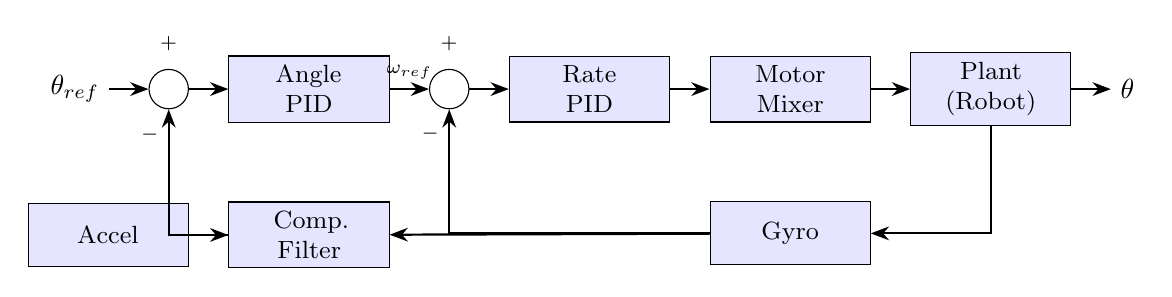
\begin{tikzpicture}[
    block/.style={rectangle, draw, fill=blue!10, text width=1.8cm, text centered, minimum height=0.8cm, font=\small},
    sum/.style={circle, draw, fill=white, minimum size=0.5cm},
    arrow/.style={-Stealth, thick},
    node distance=0.8cm
]

% Input
\node (ref) {$\theta_{ref}$};

% Angle loop
\node[sum, right=0.5cm of ref] (sum1) {};
\node[block, right=0.5cm of sum1] (pid1) {Angle\\PID};

% Rate loop
\node[sum, right=0.5cm of pid1] (sum2) {};
\node[block, right=0.5cm of sum2] (pid2) {Rate\\PID};

% Mixer and plant
\node[block, right=0.5cm of pid2] (mixer) {Motor\\Mixer};
\node[block, right=0.5cm of mixer] (plant) {Plant\\(Robot)};

% Output
\node[right=0.5cm of plant] (out) {$\theta$};

% Sensors
\node[block, below=1cm of mixer] (gyro) {Gyro};
\node[block, below=1cm of pid1] (filter) {Comp.\\Filter};
\node[block, left=0.5cm of filter] (accel) {Accel};

% Arrows
\draw[arrow] (ref) -- (sum1);
\draw[arrow] (sum1) -- (pid1);
\draw[arrow] (pid1) -- node[above, font=\scriptsize] {$\omega_{ref}$} (sum2);
\draw[arrow] (sum2) -- (pid2);
\draw[arrow] (pid2) -- (mixer);
\draw[arrow] (mixer) -- (plant);
\draw[arrow] (plant) -- (out);

% Feedback paths
\draw[arrow] (plant) |- (gyro);
\draw[arrow] (gyro) -| (sum2) node[pos=0.9, left, font=\scriptsize] {$-$};
\draw[arrow] (gyro) -- (filter);
\draw[arrow] (accel) -- (filter);
\draw[arrow] (filter) -| (sum1) node[pos=0.9, left, font=\scriptsize] {$-$};

% Labels
\node[above=0.1cm of sum1, font=\scriptsize] {$+$};
\node[above=0.1cm of sum2, font=\scriptsize] {$+$};

\end{tikzpicture}
\caption{Flight Control Loop Block Diagram}
\label{fig:control_loop}
\end{figure}

\subsection{Inputs and Outputs}

\begin{table}[H]
\centering
\caption{FC4 Inputs and Outputs}
\label{tab:fc4_io}
\begin{tabular}{@{}llll@{}}
\toprule
\textbf{Signal} & \textbf{Type} & \textbf{Range} & \textbf{Description} \\
\midrule
\multicolumn{4}{l}{\textit{Sensor Inputs}} \\
Accel\_XYZ & I2C/SPI & $\pm$16\,g & 3-axis acceleration \\
Gyro\_XYZ & I2C/SPI & $\pm$2000\,$^\circ$/s & 3-axis angular rate \\
\midrule
\multicolumn{4}{l}{\textit{RC Inputs}} \\
RC\_Throttle & PWM & 1000\,{}--2000\,$\mu$s & Throttle command \\
RC\_Roll & PWM & 1000\,{}--2000\,$\mu$s & Roll command \\
RC\_Pitch & PWM & 1000\,{}--2000\,$\mu$s & Pitch command \\
RC\_Yaw & PWM & 1000\,{}--2000\,$\mu$s & Yaw command \\
RC\_Mode & PWM & 1000\,{}--2000\,$\mu$s & Mode switch \\
\midrule
\multicolumn{4}{l}{\textit{Control Outputs}} \\
Motor\_PWM[4] & PWM & 1000\,{}--2000\,$\mu$s & Flight motor commands \\
Drive\_PWM[2] & PWM & 1000\,{}--2000\,$\mu$s & Drive motor commands \\
\midrule
\multicolumn{4}{l}{\textit{Status Outputs}} \\
Telemetry & UART & 115200\,baud & State data to ground station \\
\bottomrule
\end{tabular}
\end{table}

\subsection{Parameters}

\textbf{Attitude Estimation:}
\begin{itemize}
    \item Complementary filter alpha: 0.98 (gyro weight)
    \item Gyro calibration offset: Measured at startup
    \item Accelerometer calibration: 6-point calibration
\end{itemize}

\textbf{PID Gains (initial estimates, require tuning):}
\begin{itemize}
    \item Roll rate: $K_p = 0.5$, $K_i = 0.3$, $K_d = 0.05$
    \item Pitch rate: $K_p = 0.5$, $K_i = 0.3$, $K_d = 0.05$
    \item Yaw rate: $K_p = 1.0$, $K_i = 0.5$, $K_d = 0.0$
    \item Roll angle: $K_p = 4.0$, $K_i = 0.0$, $K_d = 0.0$
    \item Pitch angle: $K_p = 4.0$, $K_i = 0.0$, $K_d = 0.0$
\end{itemize}

\textbf{Control Loop Rates:}
\begin{itemize}
    \item Sensor read: 1000\,Hz
    \item Rate PID: 1000\,Hz
    \item Angle PID: 500\,Hz
    \item Telemetry: 50\,Hz
\end{itemize}

\subsection{Development Plan}

\begin{enumerate}
    \item Set up Teensy development environment (Arduino IDE or PlatformIO)
    \item Read IMU data over I2C and verify values
    \item Implement complementary filter and verify attitude estimation
    \item Implement rate PID controller
    \item Test rate control on single-axis gimbal jig
    \item Implement angle PID controller
    \item Implement motor mixing for X-quad configuration
    \item Integrate RC receiver input
    \item Conduct tethered flight tests
    \item Tune PID gains through flight testing
\end{enumerate}

\subsection{Test Plan}

\begin{table}[H]
\centering
\caption{FC4 Test Plan}
\label{tab:fc4_tests}
\begin{tabular}{@{}lll@{}}
\toprule
\textbf{Test} & \textbf{Method} & \textbf{Success Criteria} \\
\midrule
IMU Accuracy & Compare to reference IMU & $<$ 2\,$^\circ$ error \\
Attitude Estimation & Rotate by known angles & $<$ 5\,$^\circ$ drift over 60\,s \\
Rate Response & Step input on gimbal & Settling time $<$ 0.5\,s \\
Angle Response & Step input on gimbal & Settling time $<$ 1\,s \\
Hover Stability & Tethered hover test & Maintains $\pm$10\,$^\circ$ for 30\,s \\
\bottomrule
\end{tabular}
\end{table}

%==============================================================================
\section{FC5: Ground Station and Telemetry Interface}
\label{sec:fc5}
%==============================================================================

\subsection{Approach and Design}

The ground station provides the operator interface and data logging capability.

\textbf{Objective:} Enable remote monitoring and control of the robot with real-time data display and logging.

\textbf{Components:}
\begin{itemize}
    \item \textbf{RC Transmitter:} Standard 6+ channel transmitter (e.g., FlySky, FrSky)
    \item \textbf{Telemetry Radio:} Serial link (433\,MHz or 915\,MHz) or USB cable for testing
    \item \textbf{Ground Station Software:} Python GUI using PyQt or tkinter
\end{itemize}

\textbf{Display Features:}
\begin{itemize}
    \item Real-time attitude display (artificial horizon)
    \item Battery voltage and current
    \item Motor outputs
    \item Transformation state
    \item Data logging to CSV files
\end{itemize}

\begin{figure}[H]
\centering
\fbox{\parbox{0.8\textwidth}{\centering\vspace{3cm}\textbf{[PLACEHOLDER: Ground Station GUI Screenshot]}\\\small Insert screenshot of telemetry display software\vspace{3cm}}}
\caption{Ground Station Software Interface}
\label{fig:gui_screenshot}
\end{figure}

\subsection{Inputs and Outputs}

\begin{table}[H]
\centering
\caption{FC5 Inputs and Outputs}
\label{tab:fc5_io}
\begin{tabular}{@{}llll@{}}
\toprule
\textbf{Signal} & \textbf{Type} & \textbf{Format} & \textbf{Description} \\
\midrule
\multicolumn{4}{l}{\textit{Incoming (from robot)}} \\
Telemetry\_Packet & Serial & See below & State data packet \\
\midrule
\multicolumn{4}{l}{\textit{Outgoing (to robot)}} \\
Command\_Packet & Serial & See below & Configuration commands \\
\bottomrule
\end{tabular}
\end{table}

\textbf{Telemetry Packet Format (20 bytes):}
\begin{lstlisting}
Byte 0-1:   Header (0xAA 0x55)
Byte 2-3:   Roll angle (int16, 0.01 deg/LSB)
Byte 4-5:   Pitch angle (int16, 0.01 deg/LSB)
Byte 6-7:   Yaw angle (int16, 0.01 deg/LSB)
Byte 8-9:   Battery voltage (uint16, mV)
Byte 10-11: Current draw (uint16, mA)
Byte 12:    Mode (0=Ground, 1=Flight, 2=Transforming)
Byte 13-16: Motor outputs (4x uint8, 0-255)
Byte 17-18: Timestamp (uint16, ms)
Byte 19:    Checksum (XOR of bytes 2-18)
\end{lstlisting}

\subsection{Parameters}

\begin{itemize}
    \item \textbf{Baud rate:} 115200\,baud
    \item \textbf{Telemetry rate:} 50\,Hz
    \item \textbf{Log file format:} CSV with timestamp
    \item \textbf{Display update rate:} 30\,Hz
\end{itemize}

\subsection{Development Plan}

\begin{enumerate}
    \item Define serial packet format
    \item Implement packet encoding on Teensy
    \item Write Python serial receiver
    \item Create basic text display of received data
    \item Add graphical attitude indicator
    \item Implement data logging to CSV
    \item Add real-time plotting capability
    \item Test range and reliability with telemetry radio
\end{enumerate}

\subsection{Test Plan}

\begin{table}[H]
\centering
\caption{FC5 Test Plan}
\label{tab:fc5_tests}
\begin{tabular}{@{}lll@{}}
\toprule
\textbf{Test} & \textbf{Method} & \textbf{Success Criteria} \\
\midrule
Packet Integrity & Send known data & 0\% packet loss over 1000 packets \\
Latency & Timestamp comparison & $<$ 50\,ms end-to-end \\
Range & Increase distance & $>$ 50\,m reliable link \\
Logging & Review saved files & All data recoverable from log \\
\bottomrule
\end{tabular}
\end{table}

%==============================================================================
\section{Data Infrastructure Development}
%==============================================================================

The data infrastructure enables information flow from sensors to the operator and supports development debugging.

\subsection{Data Flow Architecture}

\begin{figure}[H]
\centering
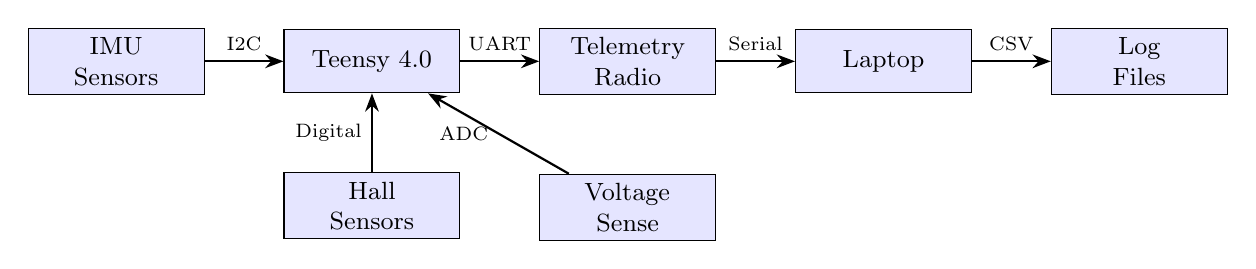
\begin{tikzpicture}[
    block/.style={rectangle, draw, fill=blue!10, text width=2cm, text centered, minimum height=0.8cm, font=\small},
    arrow/.style={-Stealth, thick},
    node distance=1cm
]

\node[block] (imu) {IMU\\Sensors};
\node[block, right=of imu] (teensy) {Teensy 4.0};
\node[block, right=of teensy] (radio) {Telemetry\\Radio};
\node[block, right=of radio] (laptop) {Laptop};
\node[block, right=of laptop] (log) {Log\\Files};

\node[block, below=of teensy] (hall) {Hall\\Sensors};
\node[block, below=of radio] (vsense) {Voltage\\Sense};

\draw[arrow] (imu) -- node[above, font=\scriptsize] {I2C} (teensy);
\draw[arrow] (teensy) -- node[above, font=\scriptsize] {UART} (radio);
\draw[arrow] (radio) -- node[above, font=\scriptsize] {Serial} (laptop);
\draw[arrow] (laptop) -- node[above, font=\scriptsize] {CSV} (log);

\draw[arrow] (hall) -- node[left, font=\scriptsize] {Digital} (teensy);
\draw[arrow] (vsense) -- node[left, font=\scriptsize] {ADC} (teensy);

\end{tikzpicture}
\caption{Data Flow Diagram}
\label{fig:data_flow}
\end{figure}

\subsection{Data Rates and Bandwidth}

\begin{table}[H]
\centering
\caption{Data Rate Requirements}
\begin{tabular}{@{}lll@{}}
\toprule
\textbf{Data Source} & \textbf{Sample Rate} & \textbf{Bytes/sec} \\
\midrule
IMU (6-axis) & 1000\,Hz & 12,000 \\
Hall sensors (4) & 100\,Hz & 400 \\
Battery voltage & 10\,Hz & 20 \\
Motor commands (6) & 500\,Hz & 3,000 \\
\midrule
Telemetry output & 50\,Hz & 1,000 \\
\bottomrule
\end{tabular}
\end{table}

At 115200\,baud, the serial link supports approximately 11.5\,kB/s, which is sufficient for the 1\,kB/s telemetry stream with margin for overhead.

\subsection{Mock Data Testing}

Before hardware is available, we will test the data pipeline using mock data:

\begin{enumerate}
    \item Generate synthetic IMU data with known motion profiles
    \item Inject synthetic data into the processing pipeline
    \item Verify attitude estimation produces expected results
    \item Test telemetry encoding/decoding with generated packets
    \item Verify logging and playback functionality
\end{enumerate}

\subsection{Hardware-in-the-Loop Testing}

Once hardware is available:
\begin{enumerate}
    \item Connect Teensy to sensors and verify raw data quality
    \item Stream real sensor data to laptop and verify reception
    \item Compare real data statistics to expected ranges
    \item Test under vibration and electromagnetic interference
\end{enumerate}

%==============================================================================
\section{System-Level Test Plan}
%==============================================================================

System-level tests evaluate the complete integrated robot against the success metrics defined in Section 2.

\subsection{Test 1: Transformation Cycle Time}

\textbf{Objective:} Verify transformation between modes completes within target time.

\textbf{Setup:} Robot on flat ground, fully charged battery, operator with RC controller.

\textbf{Procedure:}
\begin{enumerate}
    \item Start in ground mode with all sensors indicating ground position
    \item Command transformation to flight mode
    \item Record time from command to flight-ready indication
    \item Command transformation back to ground mode
    \item Record time from command to ground-ready indication
\end{enumerate}

\textbf{Success Criteria:} Full ground-to-flight-to-ground cycle $<$ 20\,s

\textbf{Metrics Recorded:}
\begin{itemize}
    \item Transformation time (each direction)
    \item Actuator current during transformation
    \item Hall sensor state transitions
\end{itemize}

\subsection{Test 2: Ground Drive Performance}

\textbf{Objective:} Verify ground mode drive speed and control.

\textbf{Setup:} Robot in ground mode on smooth floor, 15\,m marked course.

\textbf{Procedure:}
\begin{enumerate}
    \item Position robot at start line
    \item Command forward drive at 75\% throttle
    \item Record time to cross 15\,m finish line
    \item Repeat 5 times for consistency
\end{enumerate}

\textbf{Success Criteria:} Average speed $\geq$ 0.8\,m/s

\textbf{Metrics Recorded:}
\begin{itemize}
    \item Transit time
    \item Motor current draw
    \item Any steering corrections required
\end{itemize}

\subsection{Test 3: Flight Hop Performance}

\textbf{Objective:} Verify flight mode can achieve horizontal distance.

\textbf{Setup:} Robot in flight mode, outdoor area with markers at 5\,m intervals.

\textbf{Procedure:}
\begin{enumerate}
    \item Position robot at start marker
    \item Arm motors and command takeoff
    \item Fly horizontally toward 5\,m marker
    \item Land and measure actual distance traveled
    \item Repeat 3 times
\end{enumerate}

\textbf{Success Criteria:} Achieves $\geq$ 5\,m horizontal displacement

\textbf{Metrics Recorded:}
\begin{itemize}
    \item Flight distance
    \item Flight duration
    \item Battery consumption
    \item Maximum altitude reached
\end{itemize}

\subsection{Test 4: Polished Aspect Evaluation (Transformation Mechanism)}

\textbf{Objective:} Evaluate the finish quality of the transformation mechanism.

\textbf{Criteria Checklist:}
\begin{itemize}
    \item[$\square$] Hinges move smoothly without binding
    \item[$\square$] No visible wobble in locked positions
    \item[$\square$] Wiring is hidden from view
    \item[$\square$] Locking detents click audibly
    \item[$\square$] No hand assistance needed for transformation
    \item[$\square$] Consistent transformation time ($\pm$1\,s)
    \item[$\square$] Mechanism survives 100 cycles without degradation
\end{itemize}

\subsection{Test 5: Full Mission Scenario}

\textbf{Objective:} Demonstrate complete operational capability.

\textbf{Scenario:} Simulate navigating through a doorway (ground mode), encountering an obstacle, transforming to flight mode, hopping over the obstacle, landing, and transforming back to ground mode.

\textbf{Setup:} Indoor space with simulated obstacle (0.5\,m height).

\textbf{Procedure:}
\begin{enumerate}
    \item Start in ground mode, drive 5\,m toward obstacle
    \item Stop and command transformation to flight mode
    \item Take off and fly over obstacle
    \item Land on opposite side
    \item Transform back to ground mode
    \item Drive 5\,m away from obstacle
\end{enumerate}

\textbf{Success Criteria:} Complete mission without manual intervention.

%==============================================================================
\section{Engineering Calculations}
%==============================================================================

This section presents the engineering calculations that justify our component selections.

\subsection{Mass Budget}

\begin{table}[H]
\centering
\caption{Estimated Mass Budget}
\label{tab:mass_budget}
\begin{tabular}{@{}lrl@{}}
\toprule
\textbf{Component} & \textbf{Mass (g)} & \textbf{Notes} \\
\midrule
Carbon fiber frame & 200 & Two 300x200x2mm plates \\
Rotor-wheel pods (x4) & 1200 & 300g each including motor \\
Linear actuators (x2) & 200 & 100g each \\
Batteries (x2) & 400 & 200g each (6S 2200mAh) \\
Electronics & 150 & Teensy, ESCs, PDB, wiring \\
Servos and misc & 100 & DS3225 x2 plus hardware \\
\midrule
\textbf{Total} & \textbf{2250} & \\
\bottomrule
\end{tabular}
\end{table}

Design margin: Target $<$ 2.5\,kg total mass.

\subsection{Motor Thrust Calculation}

For stable hover, total thrust must exceed weight. For agile flight, we target a thrust-to-weight ratio of 2:1.

\textbf{Required total thrust:}
\begin{equation}
T_{total} = 2 \times m \times g = 2 \times 2.5\,\text{kg} \times 9.81\,\text{m/s}^2 = 49.1\,\text{N}
\end{equation}

\textbf{Required thrust per motor:}
\begin{equation}
T_{motor} = \frac{T_{total}}{4} = \frac{49.1\,\text{N}}{4} = 12.3\,\text{N} \approx 1250\,\text{g}
\end{equation}

\textbf{Selected motor analysis:}

The 2812 Pro 1100\,KV motor with 8-inch propeller produces approximately 800\,g thrust at full throttle according to manufacturer data. This gives:

\begin{equation}
\text{T/W ratio} = \frac{4 \times 800\,\text{g}}{2500\,\text{g}} = \frac{3200}{2500} = 1.28
\end{equation}

This is below our target of 2.0. \textbf{Mitigation options:}
\begin{enumerate}
    \item Upgrade to 9-inch propellers (estimated 1000\,g/motor) $\rightarrow$ T/W = 1.6
    \item Reduce total mass through design optimization
    \item Accept lower agility for initial prototype
\end{enumerate}

For the initial prototype, we will proceed with T/W = 1.28 and verify hover stability before considering upgrades.

\subsection{Servo Torque Calculation}

The transformation servos must lift the rotor-wheel pod mass against gravity.

\textbf{Pod mass:} $m_{pod} = 300\,\text{g} = 0.3\,\text{kg}$

\textbf{Arm length to center of mass:} $r = 150\,\text{mm} = 0.15\,\text{m}$

\textbf{Required torque (worst case, arm horizontal):}
\begin{equation}
\tau = m_{pod} \times g \times r = 0.3\,\text{kg} \times 9.81\,\text{m/s}^2 \times 0.15\,\text{m} = 0.44\,\text{Nm}
\end{equation}

Converting to kg-cm:
\begin{equation}
\tau = 0.44\,\text{Nm} \times \frac{100\,\text{cm}}{1\,\text{m}} \times \frac{1\,\text{kg}}{9.81\,\text{N}} = 4.5\,\text{kg-cm}
\end{equation}

\textbf{Selected servo:} DS3225 rated at 25\,kg-cm

\textbf{Safety factor:}
\begin{equation}
SF = \frac{25}{4.5} = 5.5
\end{equation}

This provides excellent margin for dynamic loads during transformation.

\subsection{Linear Actuator Force Calculation}

The linear actuators assist the servos in transformation. We analyze the force required.

Assuming the actuator pushes on the arm at a 45$^\circ$ angle to the pivot:

\textbf{Mechanical advantage:} Approximately 1.5 based on geometry

\textbf{Required actuator force:}
\begin{equation}
F_{act} = \frac{m_{pod} \times g}{MA} \times SF = \frac{0.3\,\text{kg} \times 9.81\,\text{m/s}^2}{1.5} \times 2 = 3.9\,\text{N}
\end{equation}

The original 60\,N actuator would seem sufficient, but this calculation ignores:
\begin{itemize}
    \item Friction in the pivot bearings
    \item Dynamic loads from acceleration
    \item Stall force derating
\end{itemize}

The BOM notes recommend upgrading to 150\,N or higher for reliable operation. We will use 150\,N actuators.

\subsection{Battery Sizing Calculation}

\textbf{Flight power consumption (estimated):}
\begin{itemize}
    \item Each motor at hover: 10\,A (estimated from motor specs)
    \item Total flight current: $4 \times 10\,\text{A} = 40\,\text{A}$
\end{itemize}

\textbf{Battery capacity:} 6S 2200\,mAh = 2.2\,Ah

\textbf{Hover time (80\% usable capacity):}
\begin{equation}
t_{hover} = \frac{0.8 \times 2.2\,\text{Ah}}{40\,\text{A}} \times 60\,\text{min/hr} = 2.6\,\text{min}
\end{equation}

This is sufficient for short hop maneuvers. With two batteries, we have 5.2 minutes total hover time.

\textbf{Battery discharge rate verification:}

Peak current (full throttle, 4 motors): $4 \times 25\,\text{A} = 100\,\text{A}$

Required C-rating:
\begin{equation}
C = \frac{100\,\text{A}}{2.2\,\text{Ah}} = 45C
\end{equation}

Selected battery: 150C rating $\rightarrow$ Max discharge = $150 \times 2.2\,\text{A} = 330\,\text{A}$

This provides excellent margin for peak demands.

\subsection{Structural Analysis}

\textbf{Carbon fiber plate bending:}

For a simply supported plate with center load:
\begin{equation}
\sigma_{max} = \frac{6 \times P \times L}{b \times t^2}
\end{equation}

Where:
\begin{itemize}
    \item $P = 25\,\text{N}$ (point load from battery)
    \item $L = 150\,\text{mm}$ (half span)
    \item $b = 200\,\text{mm}$ (width)
    \item $t = 2\,\text{mm}$ (thickness)
\end{itemize}

\begin{equation}
\sigma_{max} = \frac{6 \times 25 \times 0.15}{0.2 \times 0.002^2} = 28.1\,\text{MPa}
\end{equation}

Carbon fiber tensile strength: $>$ 500\,MPa

Safety factor: $>$ 17 (more than adequate)

%==============================================================================
\section{Bill of Materials}
%==============================================================================

Table~\ref{tab:bom} presents the complete bill of materials for the transformer robot.

\begin{table}[H]
\centering
\caption{Bill of Materials}
\label{tab:bom}
\small
\begin{tabular}{@{}p{3.5cm}p{4cm}crrp{2cm}@{}}
\toprule
\textbf{Component} & \textbf{Description} & \textbf{Qty} & \textbf{Unit} & \textbf{Total} & \textbf{Source} \\
\midrule
\multicolumn{6}{l}{\textit{Actuators}} \\
Servo DS3225 & 25kg torque, 180 deg & 2 & \texteuro14.39 & \texteuro28.78 & AliExpress \\
Motor 2812 Pro & 1100KV brushless & 4 & \texteuro11.00 & \texteuro44.00 & AliExpress \\
Motor 5010 & 360KV brushless (drive) & 2 & \texteuro17.29 & \texteuro34.58 & AliExpress \\
Linear Actuator & 12V, 100mm, 150N & 2 & \texteuro17.70 & \texteuro35.40 & AliExpress \\
\midrule
\multicolumn{6}{l}{\textit{Motor Control}} \\
4-in-1 ESC & 45A brushless & 1 & \texteuro30.00 & \texteuro30.00 & GetFPV \\
Bidirectional ESC & 35A brushless & 2 & \texteuro10.29 & \texteuro20.58 & Amazon \\
DRV8871 & H-bridge driver & 2 & \texteuro3.15 & \texteuro6.30 & Amazon \\
\midrule
\multicolumn{6}{l}{\textit{Flight Components}} \\
Propellers & 8x4.5 or 9x5 (CW/CCW) & 4 & \texteuro0.92 & \texteuro3.68 & Amazon \\
\midrule
\multicolumn{6}{l}{\textit{Structure}} \\
Carbon Fiber Plate & 2mm, 300x200mm & 2 & \texteuro80.00 & \texteuro160.00 & Amazon \\
Bearings & MR128-2RS, 12x8x3.5mm & 6 & \texteuro1.20 & \texteuro7.20 & Amazon \\
3D Printed Parts & PLA filament & 1 & \texteuro20.00 & \texteuro20.00 & Local \\
\midrule
\multicolumn{6}{l}{\textit{Power}} \\
6S LiPo Battery & 2200mAh, 150C & 2 & \texteuro25.00 & \texteuro50.00 & Amazon \\
Buck Converter & 22V to 5V & 1 & \texteuro2.00 & \texteuro2.00 & AliExpress \\
Buck Converter & 22V to 12V & 1 & \texteuro2.00 & \texteuro2.00 & AliExpress \\
\midrule
\multicolumn{6}{l}{\textit{Electronics}} \\
Teensy 4.0 & Microcontroller & 1 & \texteuro30.40 & \texteuro30.40 & PJRC \\
Custom PCB & Power distribution & 1 & \texteuro8.31 & \texteuro8.31 & JLCPCB \\
XT60 Connectors & Power connectors & 10 & \texteuro2.00 & \texteuro20.00 & Amazon \\
IMU (MPU6050) & 6-axis sensor & 1 & \texteuro5.00 & \texteuro5.00 & Amazon \\
Misc Electronics & Wire, headers, etc. & 1 & \texteuro15.00 & \texteuro15.00 & Various \\
\midrule
\multicolumn{4}{r}{\textbf{Total (EUR)}} & \textbf{\texteuro523.23} & \\
\multicolumn{4}{r}{\textbf{Total (CAD, approx)}} & \textbf{\$760} & \\
\bottomrule
\end{tabular}
\end{table}

\textbf{Budget Notes:}
\begin{itemize}
    \item Course budget: \$200 CAD from Digikey/McMaster/Amazon
    \item Remaining cost: \$560 CAD (personal funds)
    \item Carbon fiber plates are the largest expense; alternatives include aluminum or 3D printed frames
    \item Some components may be available from the parts library
\end{itemize}

%==============================================================================
\section{Preliminary Design}
%==============================================================================

This section provides placeholder figures for CAD and circuit documentation.

\begin{figure}[H]
\centering
\fbox{\parbox{0.8\textwidth}{\centering\vspace{3cm}\textbf{[PLACEHOLDER: Transformation Sequence Diagram]}\\\small Insert sequence of images showing ground-to-flight transformation\vspace{3cm}}}
\caption{Transformation Sequence: Ground Mode to Flight Mode}
\label{fig:transform_sequence}
\end{figure}

\begin{figure}[H]
\centering
\fbox{\parbox{0.8\textwidth}{\centering\vspace{3cm}\textbf{[PLACEHOLDER: Signal Routing Schematic]}\\\small Insert circuit schematic showing signal connections between Teensy, sensors, and ESCs\vspace{3cm}}}
\caption{Circuit Schematic: Signal Routing}
\label{fig:circuit_signal}
\end{figure}

\begin{figure}[H]
\centering
\fbox{\parbox{0.8\textwidth}{\centering\vspace{3cm}\textbf{[PLACEHOLDER: PCB Layout]}\\\small Insert PCB layout image from KiCad/JLCPCB\vspace{3cm}}}
\caption{Custom PCB Layout for Power Distribution}
\label{fig:pcb_layout}
\end{figure}

%==============================================================================
\section*{References}
%==============================================================================

\begin{enumerate}
    \item E. Sabree et al., ``Multi-Modal Mobility Morphobot (M4) with appendage repurposing for locomotion plasticity enhancement,'' \textit{Nature Communications}, 2023.
    \item Caltech Autonomous Systems and Technologies, M4 Robot Project Documentation.
    \item EMAX Motor Specifications, 2812 Pro Series Datasheet.
    \item Teensy 4.0 Technical Reference Manual, PJRC.
\end{enumerate}

\end{document}
